\section{Auswertung}
\label{sec:Auswertung}

\subsection{Untersuchung der Filterkurve}

Für die Filterkurve wurden die folgenden \autoref{tab:tab1} Messadaten aufgenommen, dabei wurde eine 10-fache Verstärkung verwendet.

\begin{table}[H]
    \centering
    \caption{Messwerte zur Filterkurve.}
    \label{tab:tab1}
    \begin{tabular}{S S}
      \toprule
      {$f \mathbin{/} \unit{\kilo\hertz} $} & {$U \mathbin{/} \unit{\milli\volt} $}  \\
      \midrule
            10.01       &   0.5     \\
            12.95       &   0.78    \\
            16.03       &   1.11    \\
            19.03       &   2.73    \\
            20.1        &   4.4     \\
            21.0        &   8.1     \\
            22.7        &   6.9     \\
            21.1        &   8.1     \\
            30.6        &   0.84    \\
            33.0        &   0.6     \\
            36.2        &   0.51    \\
            38.3        &   0.46    \\
            40.0        &   0.4     \\
      \bottomrule
    \end{tabular}
\end{table}

Die Messwerte aus \autoref{tab:tab1} sind auch in \autoref{fig:Graph_a} dargestellt.

\begin{figure}[H]
    \centering
    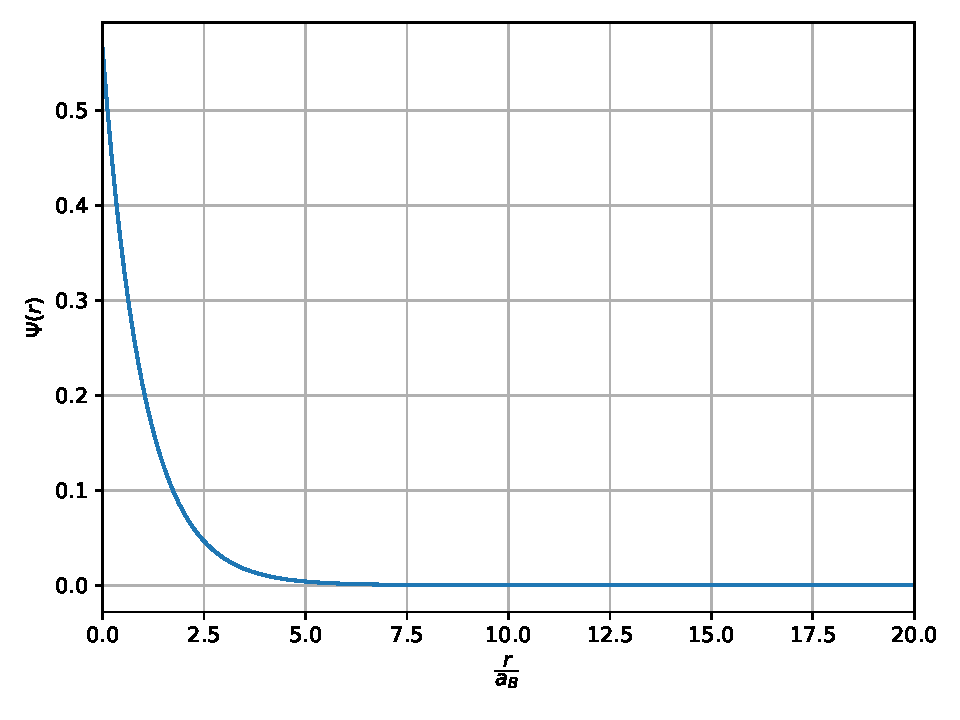
\includegraphics{build/Graph_a.pdf}
    \caption{Filterkurve der Brückenschaltung}
    \label{fig:Graph_a}
\end{figure} 

Es wurde versucht mit $ scipy$ eine Lorentzkurve der Form \eqref{eq:Lorentzkurve}, sowie eine Gaußverteilung der Form \eqref{eq:gauß} zu fitten, jedoch konnten keine Parameter, die zu den Messdaten passen gefunden werden

\begin{equation}
    f_l(v) = \frac{a}{(v^2-v_0^2)^2 + {\gamma}^2 v_0^2}
    \label{eq:Lorentzkurve}
\end{equation}

\begin{equation}
    f_g(v) = b \cdot \exp{\frac{(v-v_0)^2}{a}} \,.
    \label{eq:gauß}
\end{equation} 

Das Maximum der Spannung wird als

\begin{equation}
    U_A = 8,1 \, \unit{\volt}
\end{equation}

bei einer Frequenz von 
\begin{equation}
    v_0 = 21,05 \, \unit{\kilo\hertz}
\end{equation}
bestimmt.

\subsection{Experiemntelle Bestimmung der Suszeptibilität}

Die Probe liegt in einem Pulver vor, deswegen ist die Dichte $ \rho_p$ geringer als wenn sie aus einem einzelnen Kristall bestehen würde.
Deswegen wird aus dem eigentlichen Querschnitt ein realer Querschnitt $Q_{real} $ berechnet, welchen die Probe hätte, wenn sie aus einem Kristall bestehen würde.
Dazu wird die Formel \eqref{eq:Qreal} verwendet
\begin{equation}
    Q_{real} = \frac{M_p}{l \rho_w} .
    \label{eq:Qreal}
\end{equation}
$M_p$ ist die Masse der Probe. $\rho_w$ ist die Dichte eines Einkristalls und $l$ die Länge der Probe.
Die Werte für die Proben sind der der folgenden \autoref{tab:tab2} angegeben.


\begin{table}[H]
    \centering
    \caption{Stoff, Länge der Probe, Masse und Dichte und realer Querschnitt der Probe.}
    \label{tab:tab2}
    \begin{tabular}{S S S S S}
      \toprule
        {$\text{Stoff}$}&{$l \mathbin{/} \unit{\centi\meter} $}&{$\text{M}_p \mathbin{/} \unit{\gram} $}&{$ \rho_w \mathbin{/} \unit{\gram} \cdot \unit{\centi\meter}^{-3}$}&{$Q_{real} \mathbin{/} \unit{\centi\meter}^{2}$}\\
        \midrule
        {$\text{Dy}_2 \text{O}_3$} & {15,5}& {14,34}&{7,81}&{0,1189}\\
        {$\text{Gd}_2 \text{O}_3$} & {15.9}& {10,20}&{7,07}&{0,8669}\\
        {$\text{Nd}_2 \text{O}_3$} & {16.0}& {7,66} &{7,24}&{0,6613}\\
      \bottomrule
    \end{tabular}
\end{table}


\begin{table}[H]
    \centering
    \caption{Messadaten für $\text{Dy}_2 \text{O}_3$.}
    \label{tab:tab3}
    \begin{tabular}{S S S S S S}
      \toprule
        {$ R_0 \mathbin{/} \unit{\ohm} $}&{$R_m \mathbin{/} \unit{\ohm} $}&{$ \Delta R \mathbin{/} \unit{\ohm}$}&{$ U_0 \mathbin{/} \unit{\volt}$}&{$U_m \mathbin{/} \unit{\volt}$}&{$\Delta U \mathbin{/} \unit{\volt}$}\\
        \midrule
        {2,67} & {1.145}&  {1.525}&{0.0615}&{0.0895}&{0.0280}\\
        {2,65} & {1.15} &   {1.5} &{0.062} &{0.057} &{0.0050}\\
        {2,61} & {0.965}&  {1.645}&{0.0605}&{0.054} &{0.0065}\\
      \bottomrule
    \end{tabular}
\end{table}

\begin{table}[H]
    \centering
    \caption{Messadaten für $\text{Gd}_2 \text{O}_3$.}
    \label{tab:tab4}
    \begin{tabular}{S S S S S S}
      \toprule
        {$ R_0 \mathbin{/} \unit{\ohm} $}&{$R_m \mathbin{/} \unit{\ohm} $}&{$ \Delta R \mathbin{/} \unit{\ohm}$}&{$ U_0 \mathbin{/} \unit{\volt}$}&{$U_m \mathbin{/} \unit{\volt}$}&{$\Delta U \mathbin{/} \unit{\volt}$}\\
        \midrule
        {2.56} & {1.785}&  {0.775}&{0.058}&{0.0595}&{0.0015}\\
        {2.5}  & { 1.81}&   {0.69} &{0.061}&{0.0585} &{0.0025}\\
        {2.55} & {1.805}&  {0.745}&{0.062}&{0.059} &{0.0030}\\
      \bottomrule
    \end{tabular}
\end{table}

\begin{table}[H]
    \centering
    \caption{Messadaten für $\text{Nd}_2 \text{O}_3$.}
    \label{tab:tab5}
    \begin{tabular}{S S S S S S}
      \toprule
        {$ R_0 \mathbin{/} \unit{\ohm} $}&{$R_m \mathbin{/} \unit{\ohm} $}&{$ \Delta R \mathbin{/} \unit{\ohm}$}&{$ U_0 \mathbin{/} \unit{\volt}$}&{$U_m \mathbin{/} \unit{\volt}$}&{$\Delta U \mathbin{/} \unit{\volt}$}\\
        \midrule
        {2.68} & {2.3} &  {0.38}&{0.061} &{0.0655}&{0.0045}\\
        {2.51} & {2.38}&  {0.13}&{0.0615}&{0.0615}&{0.0}\\
        {2.6}  & {2.3} &  {0.3} &{0.0645}&{0.063} &{0.0015}\\
      \bottomrule
    \end{tabular}
\end{table}

Die Tabellen \autoref{tab:tab3}, \autoref{tab:tab4} und \autoref{tab:tab5} zeigen die Messwerte für die drei verschiedenen Proben.\\
Nach \eqref{eq:widsus} kann die Suszeptibilität durch $ \Delta R$ ausgrechnet werden und nach \eqref{eq:spannsussimp} über $\Delta U$.
Die Ergebnisse sind in \autoref{tab:tab6} eingetragen.

\begin{table}[H]
    \centering
    \caption{Experiemntelle Werte für die Suszeptibilität.}
    \label{tab:tab6}
    \begin{tabular}{S S S S S S}
      \toprule
        {$ R_0 \mathbin{/} \unit{\ohm} $}&{$R_m \mathbin{/} \unit{\ohm} $}&{$ \Delta R \mathbin{/} \unit{\ohm}$}&{$ U_0 \mathbin{/} \unit{\volt}$}&{$U_m \mathbin{/} \unit{\volt}$}&{$\Delta U \mathbin{/} \unit{\volt}$}\\
        \midrule
        {2.68} & {2.3} &  {0.38}&{0.061} &{0.0655}&{0.0045}\\
        {2.51} & {2.38}&  {0.13}&{0.0615}&{0.0615}&{0.0}\\
        {2.6}  & {2.3} &  {0.3} &{0.0645}&{0.063} &{0.0015}\\
      \bottomrule
    \end{tabular}
\end{table}
